\documentclass[a4paper,11pt]{report}
\usepackage{color}
\usepackage{graphicx}
\usepackage{subcaption}
\usepackage{wrapfig}
\usepackage[export]{adjustbox}
\usepackage{geometry}
\usepackage{setspace}
\doublespacing
\geometry{legalpaper, portrait, margin=2cm}
\begin{document}
\title{Attempt 1}
\author{Samuel Mendis}
\date{\today}
\maketitle
\tableofcontents
\chapter{Introduction}
This is the introduction.

\section{Literary Review}

\subsection{LaTex Software}
\label{sec1}

This is where I write about how much I read.
I \textbf{dislike} this software at the moment it is very cumbersome.


\chapter{Method}

\section{LaTex Software}

\subsection{benefits}
\
This software is very {\color{red}good} at separating out section, subsections etc. I take back what I said in \ref{sec1} on page %This is how I make comments which arent shown on the pdf
\pageref{sec1} about how cumbersome it is. The benefits are outlined below:
\begin{enumerate}
\item The ability to view everything so clearly
\item The way the structures are set out
\begin{itemize}
\item[-] The chapters
\item[-] The Title page
\end{itemize}
\item The simplicity of the software
\item The ability to use symbols such as \%
\end{enumerate}

\chapter{Learning}
\section{Tables}
I will be practicing tables in this section
\subsection{Practice}
\begin{tabular}{|c|c|c|} 
\hline
 &Fruits & Vegetables\\
 \hline
 Orange & Yes & No\\
 \hline
 Tomato & Yes & No\\
 \hline
 Sweet Potato & No & Yes\\
 \hline
 \end{tabular}
 \subsection{Practical}
 
 First Table:\\ 
 
 \begin{tabular}{l|r|r}
 Item&Quantity&Price(\$)\\
 \hline
 Nails&500&0.34\\
 
 Wooden boards&100&4.00\\
 
 \end{tabular}\\
 \\
 \\
 Second Table:\\
 
 \begin{tabular}{c|ccc}
 &&Year&\\
 \cline{2-4}
 City&2006&2007&2008\\
 \hline
 London&45789&46551&51298\\
 Berlin&34549&32543&29870\\
 \end{tabular}
  \pagebreak
  
 \section{Figures}
\label{sec2}
In this section I will be trying to manipulate figures so that they will occur in the correct place. I will have 3 figures to try and use, the back figure should be wrapped by this paragraph, the other two figures displayed below as a singular figure.
\begin{wrapfigure}{l}{0.5\textwidth}
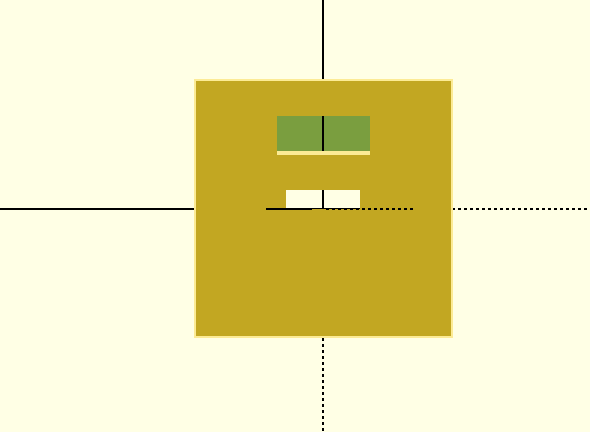
\includegraphics[width=1\linewidth]{Back}
\caption{My test image - Back of ageing setup}
\end{wrapfigure}\noindent I will have 3 figures to try and use, the back figure should be wrapped by this paragraph, the other two figures displayed below as a singular figure. This process is taking a lot longer than planned as it is just not working. Make sure to be careful when using the function "incldegraphics" as for it to work you need to specify "linewidth" not "textwidth".
  \\
  \\
  \\
  \\

 
\begin{figure}[h]

\begin{subfigure}{0.5\textwidth}
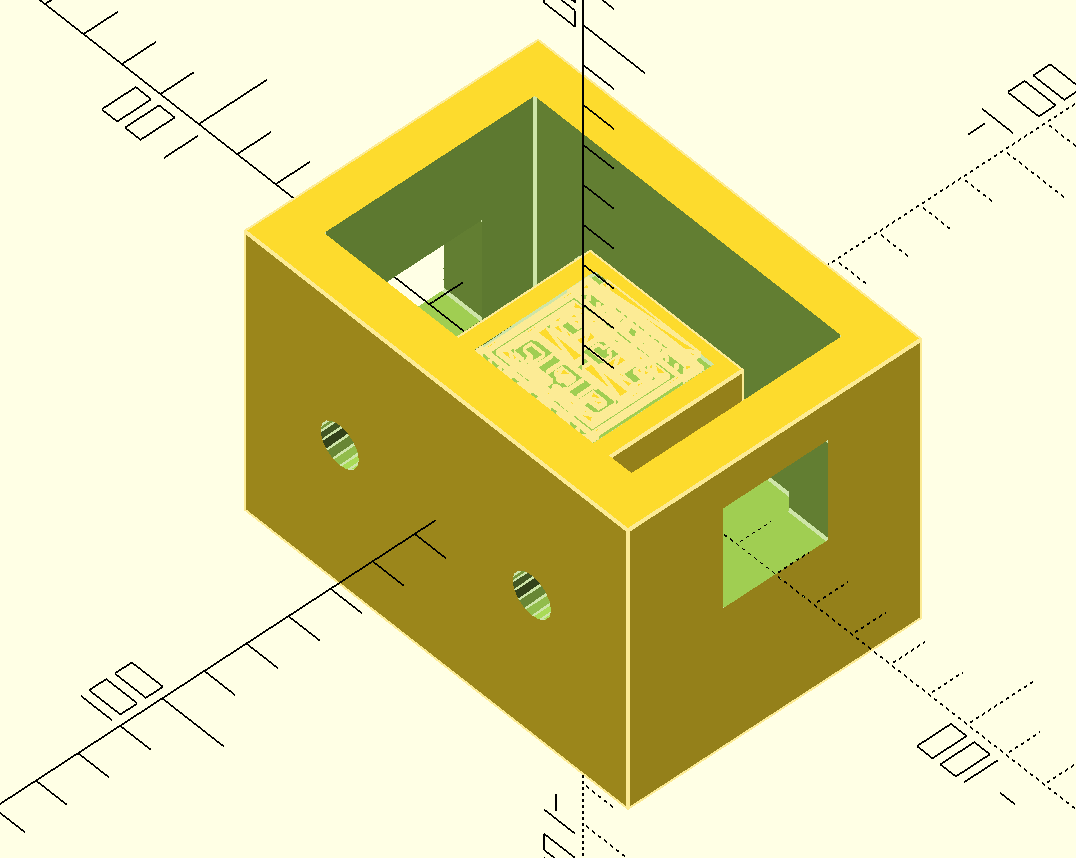
\includegraphics[width=0.9\linewidth, height=5cm]{Iso} 
\caption{Isometric View}
\label{fig:subim1}
\end{subfigure}
\begin{subfigure}{0.5\textwidth}
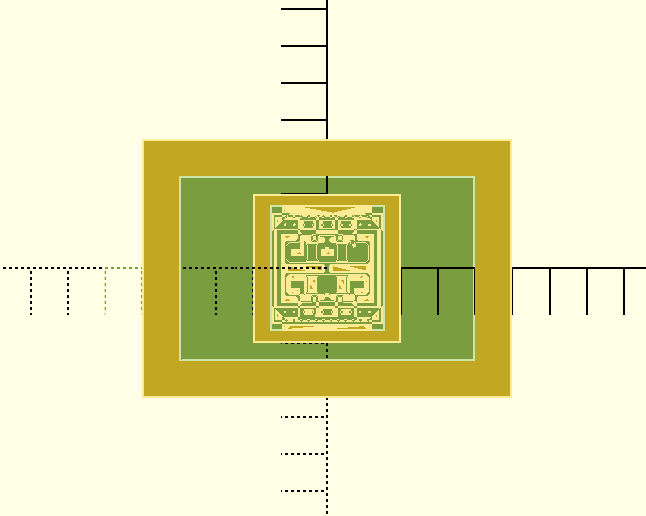
\includegraphics[width=0.9\linewidth, height=5cm]{Plan}
\caption{Plan View}
\label{fig:subim2}
\end{subfigure}

\caption{Figure showing plan and isometric views of box}
\label{fig:image2}
\end{figure}

 
 
 
\end{document}